\documentclass[11pt]{beamer}
%
% Choose how your presentation looks.
%
% For more themes, color themes and font themes, see:
% http://deic.uab.es/~iblanes/beamer_gallery/index_by_theme.html
%
	\definecolor{bostonuniversityred}{rgb}{0.8, 0.0, 0.0}
\mode<presentation>
{
  \usetheme{Madrid}      % or try Darmstadt, Madrid, Warsaw, ...
  \usecolortheme{beaver} % or try albatross, beaver, crane, ...
  \usefonttheme{default}  % or try serif, structurebold, ...
  \setbeamertemplate{navigation symbols}{}
  \setbeamertemplate{caption}[numbered]
} 
%\usepackage{pifont}
\usepackage{listings}
\usepackage{euler}
\usepackage{tikz}
\usetikzlibrary{bayesnet}
\usetikzlibrary{arrows}
\usepackage{bbm}
\usetheme[secheader]{Boadilla}
\usecolortheme[named=bostonuniversityred]{structure}
\usepackage[bookmarks]{hyperref}
\usepackage[backend=bibtex]{biblatex}
\usepackage[a-3u]{pdfx} 
\setbeamercolor{title}{parent=author in head/foot}
\usepackage{braket}
\usepackage{amsmath,amsfonts,amsthm,bm}
\addbibresource{bibliography.bib}
\newtheorem*{remark}{Remark}
\usepackage[italian]{babel}
\usepackage[utf8x]{inputenc}
\usebackgroundtemplate{\includegraphics[width=\paperwidth]{Pic/Cover_image.png}}
\title[Review]{Time series}
\author{Marzio De Corato}
\date{\today}

\begin{document}

\begin{frame}
\vspace{+6.9 cm}  \titlepage
\end{frame}

\usebackgroundtemplate{ } 

\begin{frame}{Time series definition \cite{brockwell2002introduction}}
\begin{alertblock}{Informal definition}
A time-series is a set of observation $x_{t}$ each one being recorder at a specific time t. 
\end{alertblock}
\begin{alertblock}{Formal definition }
A time series model for the observed data ${x}_{t}$ is a specification of the joint distribution (or possibile only the mens covariance) of a sequence of random variable ${X}_{t}$ of which ${x}_{t}$ is postulated to be a realization
\end{alertblock}
\begin{exampleblock}{A binary process}
Consider the sequence of iid random variables, with $P[X_{t}=1]=p$ and $P[X_{t}=-1]=1-p$
\end{exampleblock}
\begin{exampleblock}{Random walk}
The random walk is obtained by cumulatevely summing iid random variables. Thus a random walk with zero mean is obtained by defining $S_{0}=0$ and $S_{t}=X_{1}+X_{2}+...+X_{t}$ for $t=1,2,..$ where ${X_{t}}$ a iid noise. 
\end{exampleblock}
\end{frame}


\begin{frame}{Stationarity, autocovariance and autocorrelation\cite{brockwell2002introduction}}
\begin{alertblock}{Mean Function}
Let ${X_{t}}$ be a time series with $E({x}_{t}^{2}< \infty$  The mean function of ${X_{t}}$ is $\mu_{X}(t)=E(X_{t})$. The covariance function of ${X_{t}}$ is $\gamma_{X}(r,s)=Cov(X_{r},X_{S})=E[(X_{r}-\mu_{X}(r))(X_{s}-\mu_{X}(s))]\quad\forall r,s$ 
\end{alertblock}
\begin{alertblock}{Weakly stationary TS}
${X_{t}}$ is weakly stationary if i) $\mu_{X}(t)$ is indipendent from time t and ii) $\gamma_{X}(t+h)$ is indipendent of t $\forall h$
\end{alertblock}
\begin{alertblock}{Autocovariance function}
At lag h the autocovariance function is defined as $\gamma_{X}(h)=Cov(X_{t+h},X_{t})$ 
\end{alertblock}
\begin{alertblock}{Autocorellation function}
At lag h the autocorrelation function is defined as $\rho(h)_{X}=\dfrac{\gamma_{X}(h)}{\gamma_{X}(0)}=Cor({X}_{t+h},{X}_{t})$ 
\end{alertblock}
\end{frame}

%\begin{frame}{Interpretabilità per le reti neurali \cite{xai_ff}}
%    \begin{center}
%     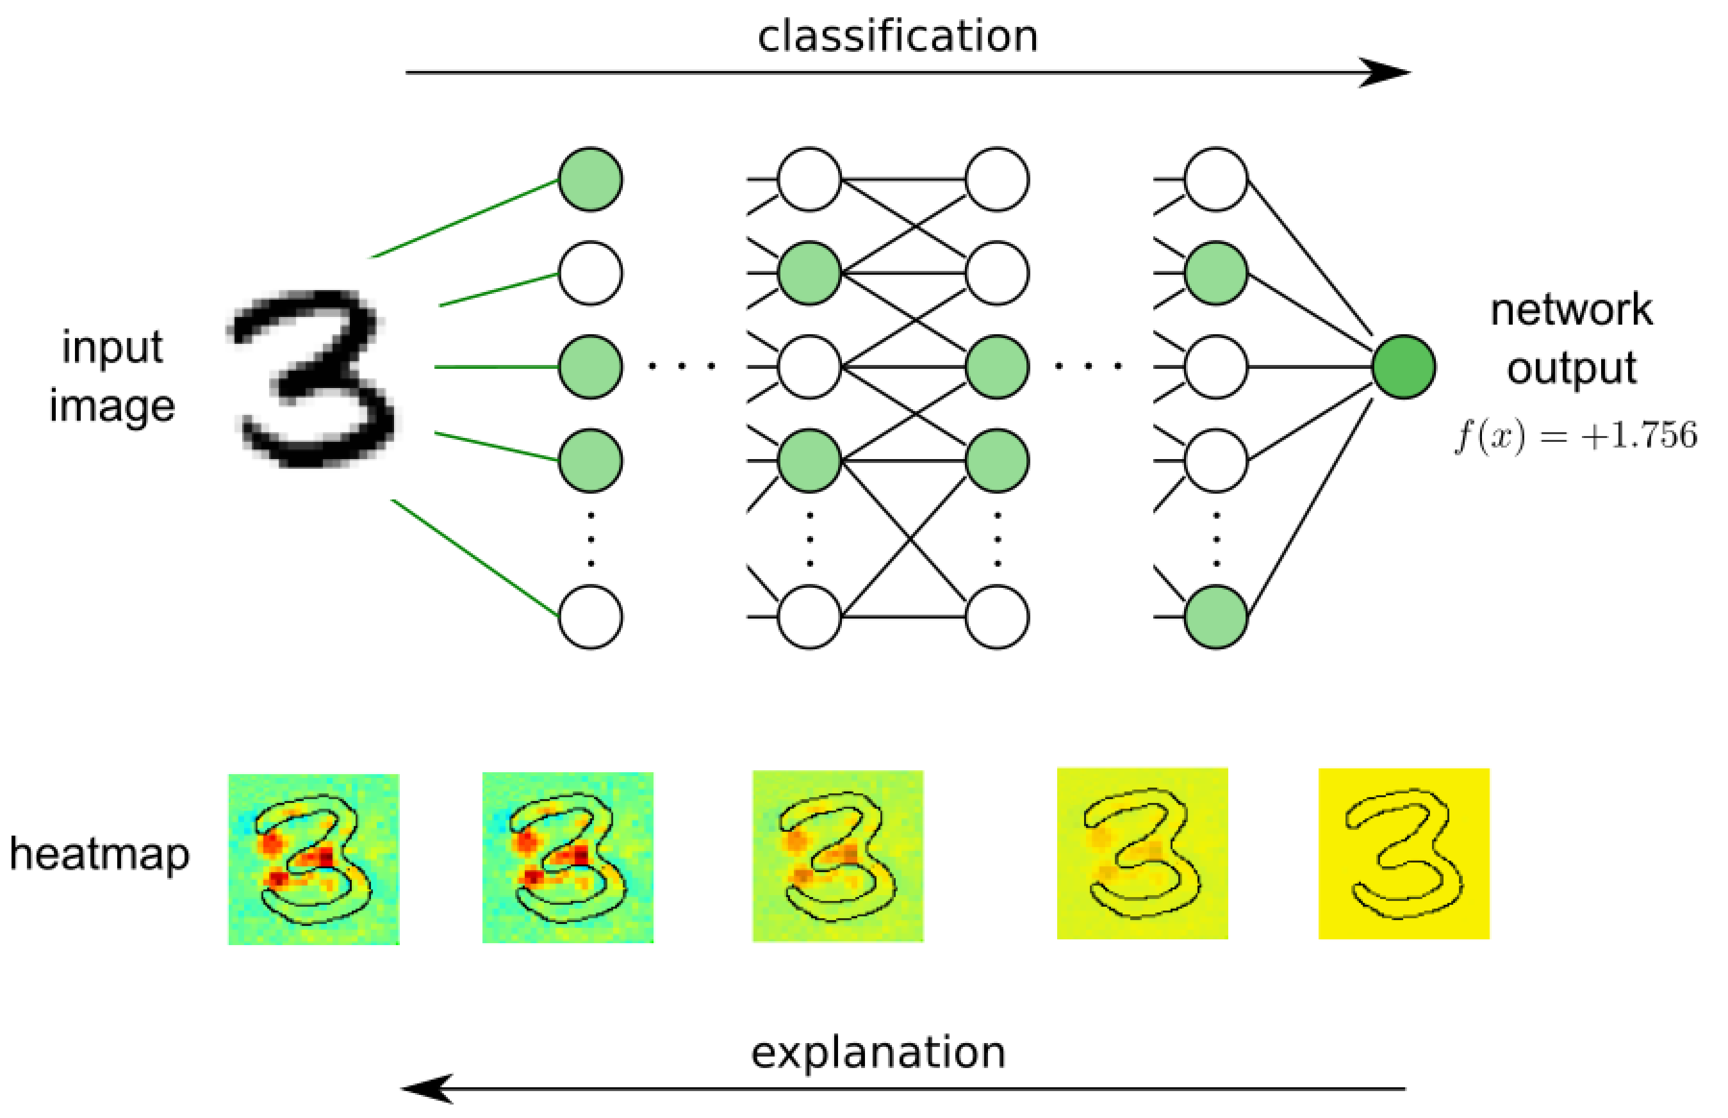
\includegraphics[width=0.6\textwidth]{Pic/XAI_nn.png}
%     \end{center}
%\end{frame}






\begin{frame}[noframenumbering,t,allowframebreaks]
\frametitle{Bibliography}
\printbibliography
\end{frame}



\end{document}
